\chapter{Applying numerical methods to the Orr-Sommerfeld equation} \label{chap:numerics}
This chapter focuses on a numerical method for finding the eigenvalues $ c $ of the Orr-Sommerfeld equation using Chebyshev polynomials. We will first introduce the Chebyshev polynomials and some of their properties before explaining how they can approximate functions and their derivatives. From there, we will discuss how we can obtain the eigenvalues of the Orr-Sommerfeld equation using the Chebyshev Tau method and how we can split the Orr-Sommerfeld equation into systems of lower-order differential equations to increase numerical accuracy.
 
\section{Chebyshev polynomials}

Chebyshev polynomials are a family of polynomials that are orthogonal with respect to the following inner product \citep{bukhari1997spectral}
\begin{equation}
    \langle f, g \rangle = \inte{1}{-1}{\frac{f g}{ \sqrt{1-z^2}}}{z}.
\end{equation}
% solve the following Sturm-Loiuville problem on the interval $ z \in (-1, 1) $ \citep{canuto2007spectral}
% \begin{equation}
%     (\sqrt{1 - z^2} T'_k(z))' + \frac{k^2}{\sqrt{1 - z^2}} T_k(z) = 0.
% \end{equation} 

The $k$-th order Chebyshev polynomial is given by
\begin{equation}
    T_k(z) = \cos{(k \theta)},\ \ z = \cos{\theta}.
\label{cheby}
\end{equation}

Specifically, if we take the inner product of two Chebyshev polynomials, we get the following result \citep{canuto2007spectral},
\begin{align}
    \langle T_i(z), T_j(z) \rangle = \inte{1}{-1}{\frac{T_i(z) T_j(z)}{\sqrt{1-z^2}}}{z} = \begin{cases}
        0,&\ \ \text{if}\ i \neq j, \\
        c_k \tfrac{\pi}{2},&\ \ \text{if}\ i = j,
    \end{cases},
    \label{chebyip}
\end{align}
where $ c_k = 2 $ if $ k = 0 $ and $ c_k = 1$ for all $ k \geq 1 $.

We've plotted the first $ 5 $ Chebyshev polynomials in Figure \ref{fig:cheby04}. From this, we can see that Chebyshev polynomials are odd when $ k $ is odd and even when $k $ is even. They also appear to be well defined at $ z = \pm 1 $. It turns out that all Chebyshev polynomials take values of $ \pm 1 $ at these endpoints \citep{canuto2007spectral}. The exact boundary values are as follows
\begin{equation}
    T_k(\pm 1) = (\pm 1)^{k},\ \ T_k'(\pm 1) = (\pm 1)^{k+1} k^2.
    \label{chebyprop}
\end{equation}
The fact that Chebyshev polynomials take such well-defined values at the endpoints of our interval for $z $ will be very useful when we come to represent the boundary conditions of the Orr-Sommerfeld equation in terms of Chebyshev polynomials in Section \ref{section:bc}.

\begin{figure}[htb!]
    \centering
    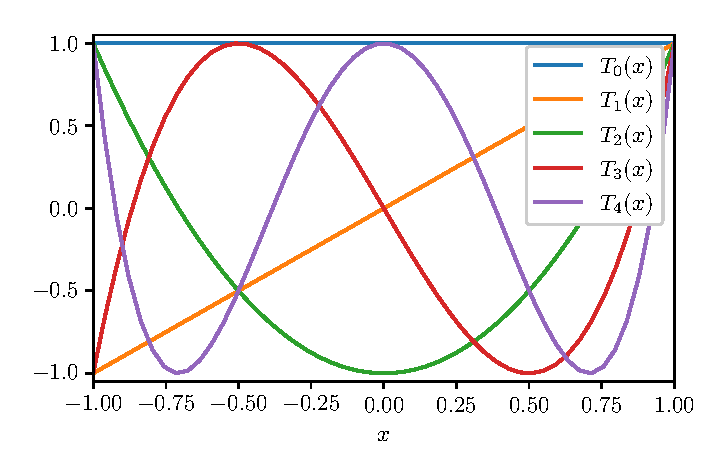
\includegraphics{figures/chebyshevs.eps}
    \caption{Chebyshev polynomials from $ N = 0, \dots, 4 $}
    \label{fig:cheby04}
\end{figure}

% They have the power series \citep{canuto2007spectral}
% \begin{equation}
%     T_k(z) = \frac{k}{2} \sum^{[k/2]}_{l=0} (-1)^k \frac{(k - l - 1)!}{l! (k - 2l)!} (2z)^{k - 2l}.
% \end{equation}

One of the useful properties of Chebyshev polynomials is the fact that we can find recursive relations relating $ T_k(z) $ of different order. Consider the trigonometric identity $ \cos((k + 1) \theta) + \cos((k - 1) \theta) = 2 \cos(\theta) \cos(k \theta) $. If we use $ \theta = \arccos z $ as defined above we end up with the following expression
\begin{gather}
    \cos((k + 1) \arccos z) + \cos((k - 1) \arccos z) = 2 \cos(\arccos z) \cos(k \arccos z).
\end{gather}

Notice that each of the terms of this expression has the form of a different order of Chebyshev polynomial. If we replace each term with its corresponding $ T_k(z) $ and rearrange, we are then left with the following recursion relation
\begin{equation}
    T_{k+1}(z) = 2 z T_k(z) - T_{k-1}(z).
\end{equation}

% This will be extremely useful in Section \ref{section:deriv} when we discuss how to represent the derivatives of a function. 

Before we move on to discussing how we will approximate our function, there is one more useful property of Chebyshev polynomials that we will need. The $k$th order Chebyshev polynomial has $ k $ zeros at the following points \citep{canuto2007spectral}
\begin{equation}
    z_i = \cos(\frac{(1+2i) \pi}{2 k}),\ \ i = 0, \dots, k - 1.
    \label{chebyzeros}
\end{equation}

We will use these in the next section for approximating integrals using the Chebyshev-Gauss quadrature.

% \textbf{gauss quadrature and gauss points from \cite{canuto2007spectral}}

\section{Approximating a function}
We express our function $ \phi $ and its derivatives as a sum of $ M + 1 $ Chebyshev polynomials
\begin{equation}
    \dv[q]{\phi(z)}{z} = \sum^M_{k=0} a_k^{(q)} T_k(z),
    \label{expansion}
\end{equation}
where $ a_k^{(q)} $ are the expansion coefficients of the representation. This function expansion approximates $ \phi $ up to a polynomial of degree $ M $.

We represent our expansion as an $ M + 1 $ dimensional vector $ \mathbf{a} $, where the $k$th component of $ \mathbf{a} $ is the corresponding $ a_k $ from our expansion.
\begin{equation}
    \mathbf{a} = \begin{pmatrix}
        a_0^{(0)} \\
        a_1^{(0)} \\
        \dots \\
        a_{M-1}^{(0)} \\
        a_M^{(0)}
    \end{pmatrix}.
    \label{coeffvec}
\end{equation}

We will now show how to approximate the function
\begin{equation}
    f(z) = \cos(z) = \sum^M_{k=0} a_k T_k(z),
    \label{cos}
\end{equation}
as a sum of Chebyshev polynomials. Note that from now on, $ a_k$ with no superscript will represent $ a_k^{(0)} $, the coefficients corresponding to the expansion of our undifferentiated function.

To calculate our $ a_k $ we multiply both sides of \eqref{cos} by $ T_i(z) / \sqrt{1 - z^2}$ and then integrate between $ -1 $ and $ 1 $. This leaves us with
\begin{align}
    \inte{1}{-1}{\frac{\cos(z) T_i(z)}{\sqrt{1-z^2}}}{z} &= \inte{1}{-1}{\qb{\sum^M_{k=0} a_k T_k(z)} \frac{T_i(z)}{\sqrt{1-z^2}}}{z} \\
    &= \sum^M_{k=0} a_k \inte{1}{-1}{\frac{T_k(z) T_i (z)}{\sqrt{1 - z^2}}}{z}.
    \label{akderiv}
\end{align}

Notice that the integral inside the sum on the right-hand side of \eqref{akderiv} corresponds to the inner product in \eqref{chebyip}. Since Chebyshev polynomials are orthogonal, we are just left with a single coefficient when $ i = k $. This leaves us with
\begin{equation}
    \inte{1}{-1}{\frac{\cos(z) T_i(z)}{\sqrt{1-z^2}}}{z} = a_i c_i \tfrac{\pi}{2},
\end{equation}
which can be rearranged to give us an explicit formula for our $ a_k $ as seen in \citet{canuto2007spectral} 
\begin{equation}
    a_k = \frac{2}{\pi c_k} \inte{1}{-1}{\frac{f(z) T_k(z)}{\sqrt{1-z^2}}}{z}.
\label{coeffexplicit}
\end{equation}
Note: the indices $ i $ and $ k $ have been swapped for consistency with how the coefficients are referenced in our expansion.

We now have a way of calculating the corresponding Chebyshev expansion of $ \cos(z)$. However, before we can implement this in Python we need a method of approximating the integral in \eqref{coeffexplicit}. To do this we will use a Chebyshev-Gauss quadrature method. We can approximate the weighted integral in \eqref{coeffexplicit} as the following sum
\begin{equation}
    \inte{1}{-1}{\frac{g(z)}{\sqrt{1-z^2}}}{z} = \sum^N_{i=0} g(z_i) w_i,
\end{equation}
where the $ z_i $ are the $ N + 1 $ zeros of $ T_{N+1}$ as stated in \eqref{chebyzeros}. It can be shown that the corresponding $ w_i $ are constant with a value of $ \pi / (N+1)$, and that the degree of precision for this approximation is $ 2N + 1 $ \citep{canuto2007spectral}. Substituting this approximation into \eqref{coeffexplicit} leaves us with the following approximation for our $ a_k$
\begin{align}
    a_k &= \frac{2}{\pi c_k} \qb{ \frac{\pi}{N+1} \sum^N_{i=0} f(z_i) \cos(\frac{k (1 + 2i) \pi}{2 (N + 1)})} \\
    &= \frac{2}{c_k (N+1)} \sum^N_{i=0} f(z_i) \cos(\frac{k (1 + 2i) \pi}{2 (N + 1)}). 
\end{align}

We have implemented this method in Python and the code written can be found in Appendix \ref{code:funcapprox}. The approximation for different numbers of polynomials can be found in Figure \ref{fig:cosapprox}. 

\begin{figure}[h!]
    \centering
    \subfloat[Approximation for $ N = 0 $]{
        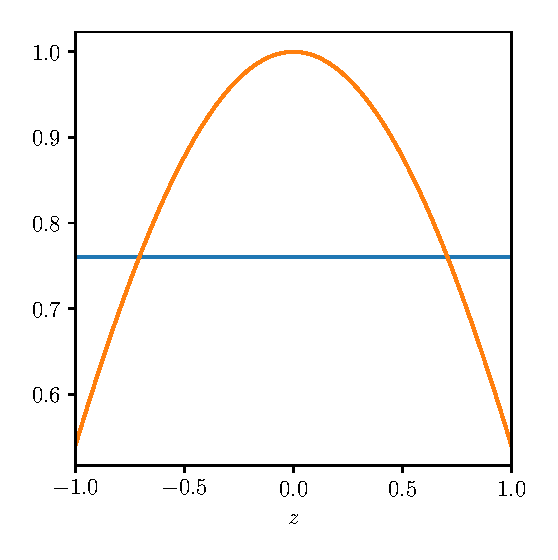
\includegraphics[width=60mm]{figures/cheby_approxN=0.eps}
    }
    \subfloat[Approximation for $ N = 1 $]{
        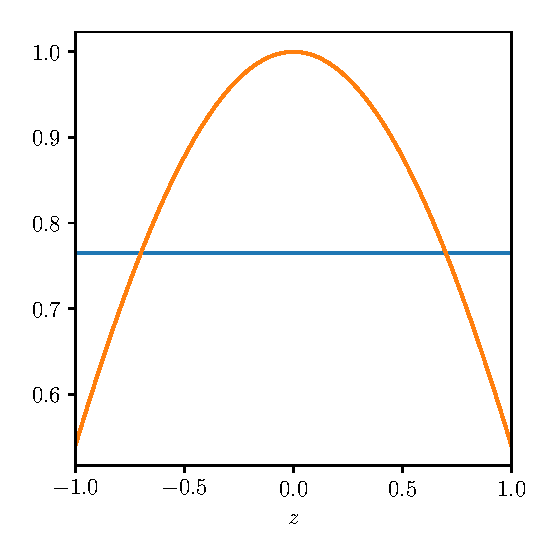
\includegraphics[width=60mm]{figures/cheby_approxN=1.eps}
    }
    \hspace{0mm}
    \subfloat[Approximation for $ N = 2 $]{
        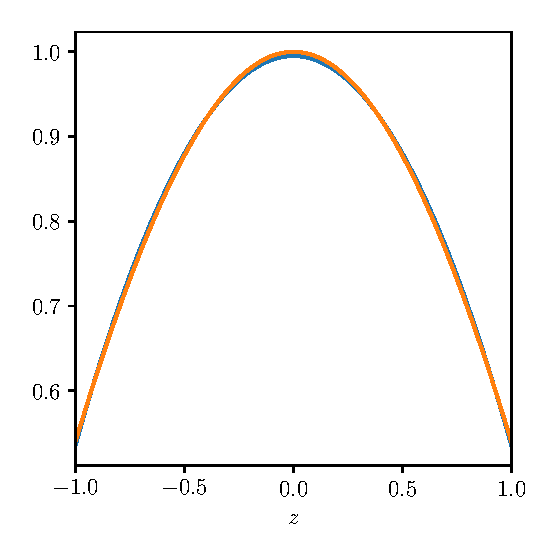
\includegraphics[width=60mm]{figures/cheby_approxN=2.eps}
    }
    \subfloat[Approximation for $ N = 5 $]{
        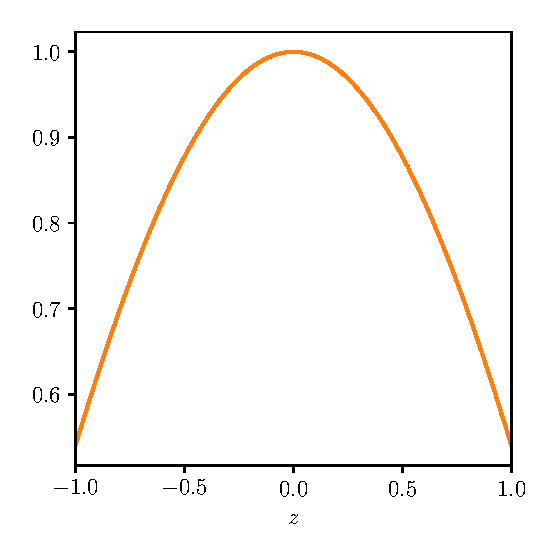
\includegraphics[width=60mm]{figures/cheby_approxN=5.eps}
    }
    \caption{The Chebyshev approximation of $ \cos(z) $ with differing numbers of polynomials (differing values of $ N$). The orange line in each plot corresponds to $ \cos(z)$, while the blue line corresponds to an approximation.}
    \label{fig:cosapprox}
\end{figure}

As can be seen, the approximation doesn't change between $ N = 0 $ and $ N = 1 $. This makes sense as the Taylor expansion of $ \cos z $ around $ z = 0 $ doesn't include any odd powers of $ z$, meaning we wouldn't expect any Chebyshev polynomials with odd order in our approximation. The Chebyshev approximation also clearly converges extremely fast, even with $ N = 2 $ there is very little difference between the approximation and the actual function. Figure \ref{fig:chebyvtaylor} shows a comparison between the second-order Chebyshev approximation of $\cos(z)$ (left), and the second-order Taylor approximation of $ \cos(z)$ (right).  

\begin{figure}[h!]
    \centering
    \subfloat[Second order Chebyshev approximation of $ \cos(z)$]{
        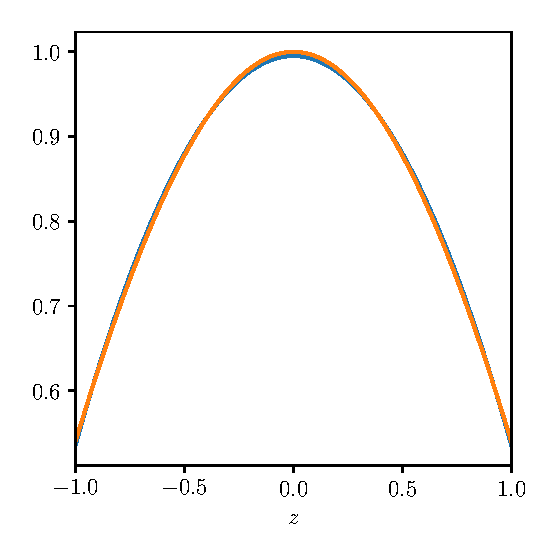
\includegraphics[width=60mm]{figures/cheby_approxN=2.eps}
    }
    \hspace{10mm}
    \subfloat[Second order Taylor approximation of $ \cos(z)$]{
        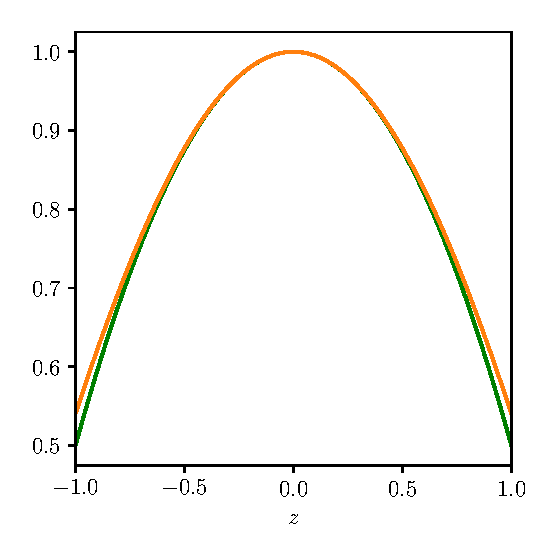
\includegraphics[width=60mm]{figures/taylor_approx.eps}
    }
    \caption{The Chebyshev approximation of $ \cos(z) $ with $ N = 2 $ blue line compared to the Taylor approximation of $ \cos(z) $ (green line).}
    \label{fig:chebyvtaylor}
\end{figure}

We can see that while the Chebyshev approximation takes an incorrect value at $ z = 0 $, there is a significant divergence between the Taylor approximation and $ \cos(z) $ at the endpoints. This implies that the Chebyshev approximation converges to $ \cos(z)$ much faster than the Taylor approximation.

Now we have a method of approximating a function, we need a method of representing the derivatives of a function in terms of some matrix $ D^m $ multiplied by our approximation vector $ \mathbf{a} $, where $m $ represents the order of derivative we are calculating. This will allow us to represent the action of differential operators on our expansion as the action of a matrix on our expansion. Calculating the form of $ D^m$ is the focus of the next section.

\section{Representing derivatives} \label{section:deriv}

Differentiating \eqref{cheby} with respect to $ z $ implies that the first derivative of the $k$-th order Chebyshev polynomial has the following form
\begin{equation}
    \dv{z} T_k(z) = \frac{-k \sin(k \arccos z)}{\sqrt{1 - z^2}} = \frac{-k \sin(k \theta)}{\sin \theta}, 
\label{chebyderiv}
\end{equation}
where $ z = \cos \theta $ as before. 

There are $ 2 $ important things to note from this definition:
\begin{enumerate}
    \item We have that $ T_k'(z) = T_{-k}'(z) $.
    \item We have the limit $ \lim_{k \rightarrow 0} T_k'(z) / k = \lim_{k \rightarrow 0} -\sin(k \theta) / \sin \theta = 0 $.
    \label{divprops}
\end{enumerate}

If  now we consider the trigonometric relation $ 2 \sin \theta \cos \theta = \sin(k+1)\theta - \sin(k-1)\theta $ we have that 
\begin{align}
    2 \cos \theta &= \frac{\sin((k+1) \theta)}{\sin \theta} - \frac{\sin((k-1) \theta)}{\sin \theta}, \\
    2 T_k(z) &= \frac{1}{k+1} T'_{k+1}(z) - \frac{1}{k-1}T'_{k-1}(z),
    \label{chebrelation}
\end{align}
which gives us a recursive relation between different orders of derivatives of Chebyshev polynomials. 

We would like to use this recursion relation to find a recursion relation between the coefficients of our undifferentiated function $ a_k$ and the coefficients of a derivative of our function $ a_k^{(q)} $. If we consider the first derivative of a perfect expansion of the form in \eqref{expansion} (i.e. the case where $ N = \infty $, we can see that the following are equivalent
\begin{equation}
    \sum^\infty_{k=0} a^{(0)}_k T_k' (z) = \dv{\p}{z} = \sum^\infty_{k = 0} a_k^{(1)} T_k.
\end{equation}

We can use this result along with the recursion relation \eqref{chebrelation} to get the following
\begin{align}
    \sum^\infty_{k=0} a_k^{(0)} T_k'(z) &= \tfrac{1}{2} \sum^\infty_{k=0} a_k^{(1)} \qb{\frac{1}{k+1} T_{k+1}'(z) - \frac{1}{k - 1} T_{k-1}'(z)} \\ 
    &= \tfrac{1}{2} \qb{\sum^\infty_{k=0} \frac{a_k^{(1)}}{k+1} T_{k+1}'(z) - \sum^\infty_{k=0} \frac{a_k^{(1)}}{k-1} T_{k-1}(z)}. \label{divsums}
\end{align}

To get a recursion relation between our coefficients, we would like to be able to compare the terms of the sums in \eqref{divsums}. Define $ n = k + 1 $ and $ m = k - 1$. If we use these as the indices in the two sums on the right of \eqref{divsums} we get the following
\begin{align}
    \sum^\infty_{k=0} a_k^{(0)} T_k'(z) &= \tfrac{1}{2} \qb{\sum^\infty_{n=1} \frac{a_{n-1}^{(1)}}{n} T_n'(z) - \sum^\infty_{m=-1} \frac{a_{m+1}^{(1)}}{m} T_m'(z)} \\
    &= \tfrac{1}{2} \qb{\sum^\infty_{k=1} \qb{\frac{a_{k-1}^{(1)}}{k} - \frac{a_{k+1}^{(1)}}{k}} T_k'(z) + a_0^{(1)} T_{-1}'(z) - \frac{a_1^{(1)}}{0} T_0(z)}. 
\end{align} 
Notice that $ T_1'(z) = T_{-1}'(z) $ in the second to last term thanks to the first of the properties of the derivative \eqref{chebyderiv} and that the last term vanishes thanks to the second of the properties of the derivative \eqref{chebyderiv}. This leaves us with
\begin{align}
    \sum^\infty_{k=0} a_k^{(0)} T_k'(z) &= \tfrac{1}{2} \sum^\infty_{k=1} \qb{\frac{c_{k-1} a_{k-1}^{(1)}}{k} - \frac{a_{k+1}^{(1)}}{k} T_k'(z)},
\intertext{From here we extract our recursion relation for our coefficients}
    2 k a_k^{(0)} &= c_{k-1} a_{k-1}^{(1)} - a_{k+1}^{(1)},\ \ k \geq 1. \label{coeffrelation}
\end{align}

We would like an expression for $ a_k^{1} $ that only uses $ a_p $ for various $p \geq 0 $. If we apply \eqref{coeffrelation} to itself we get 
\begin{align}
    c_{k - 1} a_{k-1}^{(1)} &= 2 k a_k + a_{k+1}^{(1)} \\
    &= 2k a_k + (2(k+2) a_{k+2} + a_{k+3}^{(1)} \\
    &= 2k a_k + 2(k+2) a_{k+2} + (2(k+4) a_{k + 4} + a_{k+5}^{(1)}) \\
    & \ \ \vdots
\end{align}

If we continue this process up to a truncation point of $ M $ polynomials, we obtain the following formula for the coefficients of the first derivative of $ \phi $ as seen in the literature \citep{canuto2007spectral, orszag1971accurate} 
\begin{equation}
    a_k^{(1)} = \frac{2}{c_k} \sum^{M}_{\substack{p = k + 1 \\ p \equiv 1\ (\text{mod } 2)}} p a_p. \label{divsum}
\end{equation}

To get higher derivatives we can just apply this method recursively. The second derivative is obtained by the following 
\begin{equation}
    a_k^{(2)} = \frac{2}{c_k} \sum^{M}_{\substack{p = k + 1 \\ p \equiv 1\ (\text{mod } 2)}} p a_p^{(1)}.
\end{equation}

Applying the sum \eqref{divsum} again, we can get an expression for the coefficients of the $2$nd derivative of $ \phi$ given by
\begin{equation}
    a^{(2)}_{k} = \frac{1}{c_k} \sum^{M}_{\substack{p = k + 2 \\ p \equiv 0\ (\text{mod } 2)}} p (p^2 - k^2) a_p.
\end{equation}

In a similar way, we can compute an expression for $ a^{(4)}_k $ given by
\begin{equation}
    a^{(4)}_k = \frac{1}{c_k} \sum^N_{\substack{p = k + 4 \\ p \equiv 0\ (\text{mod } 2)}} p [p^2 (p^2 - 4)^2 - 3 k^2 p^4 + 3 k^4 p^2 - k^2 (k^2 - 4)^2] a_k.
    \label{d4expansion}
\end{equation}

It is clear that for large $ p $ and $ k $, \eqref{d4expansion} grows extremely fast. This means that numerically we can lose significance as $ M $ becomes large. To reduce this, \cite{herbert1977neutrale} suggested that the substitution $ q = p - k $ be used inside the brackets. This transforms \eqref{d4expansion} into
\begin{equation}
    a^{(4)}_k = \frac{1}{c_k} \sum^N_{\substack{p = k + 4 \\ p \equiv 0\ (\text{mod } 2)}} p [q^4 (q^2 - 8) + k q^3 (6 q^2 - 32) + (12 k^2 q^2 + 8 k^3 q)(q^2 - 4) + 16 q^2 + 32 kq] a_k.
    \label{qd4expansion}
\end{equation}

We can then represent the coefficients of a derivative of $ \p $ by multiplying our vector $ \mathbf{a} $ by an $ (M + 1) \cross (M + 1) $ matrix $ D^n $

For $ n = 1 $, we have
\begin{equation}
D = \begin{pmatrix}
    0 & 1 & 0 & 3 & 0 & 5 & 0 & 7 & 0 & \dots\\
    0 & 0 & 4 & 0 & 8 & 0 & 12 & 0 & 16 & \dots\\
    0 & 0 & 0 & 6 & 0 & 10 & 0 & 14 & 0 & \dots\\
    0 & 0 & 0 & 0 & 8 & 0 & 12 & 0 & 16 & \dots\\
    0 & 0 & 0 & 0 & 0 & 10 & 0 & 14 & 0 & \dots\\
    0 & 0 & 0 & 0 & 0 & 0 & 12 & 0 & 16 & \dots\\
    \ds & \ds & \ds & \ds & \ds & \ds & \ds & \ds & \ds & \ds 
\end{pmatrix}.
\label{D}
\end{equation}

For $ n = 2 $, we have
\begin{equation}
D^2 = \begin{pmatrix}
    0 & 0 & 4 & 0 & 32 & 0 & 108 & 0 & 256 & \dots\\
    0 & 0 & 0 & 24 & 0 & 120 & 0 & 336 & 0 & \dots \\
    0 & 0 & 0 & 0 & 48 & 0 & 192 & 0 & 480 & \dots \\
    0 & 0 & 0 & 0 & 0 & 80 & 0 & 280 & 0 & \ds\\
    0 & 0 & 0 & 0 & 0 & 0 & 120 & 0 & 384 & \ds\\
    0 & 0 & 0 & 0 & 0 & 0 & 0 & 168 & 0 & \ds\\
    \dots & \dots & \dots & \dots & \dots & \dots & \dots & \dots & \ds & \ds
\end{pmatrix}.
\label{D2}
\end{equation}

For $ n = 4 $, we have
\begin{equation}
    D^4 = \begin{pmatrix}
        0 & 0 & 0 & 0 & 192 & 0 & 4608 & 0 & 38400 & \ds\\
        0 & 0 & 0 & 0 & 0 & 1920 & 0 & 26880 & 0 & \ds\\
        0 & 0 & 0 & 0 & 0 & 0 & 5760 & 0 & 61440 & \ds\\
        0 & 0 & 0 & 0 & 0 & 0 & 0 & 13440 & 0 & \ds\\
        0 & 0 & 0 & 0 & 0 & 0 & 0 & 0 & 26880 & \ds\\
        0 & 0 & 0 & 0 & 0 & 0 & 0 & 0 & 0 & \ds\\
        \ds & \ds & \ds & \ds & \ds & \ds & \ds & \ds & \ds & \ds
    \end{pmatrix}.
    \label{D4}
\end{equation}

Notice that $ D^2 $ and $ D^4 $ are in fact multiples of $ D $. This means in theory we can get any derivative of $ \p $ we want. 

These matrices are implemented in Python in the code in Appendix \ref{code:tau_matrices}. We can then test them by multiplying the coefficients of our computed approximation for $ \cos(z) $ by the matrices $ D, D^2, D^4$ to get the coefficients of the expansion of our derivatives. Note that since $ D^4$ is all zeroes if $ N \leq 4 $ we need to compute an approximation to $ \cos(z) $ that is of a higher order than order $ 4 $. Figure \ref{fig:cosderivapprox} shows the original approximation for $ N = 8 $, along with the approximation for the first, second and fourth derivatives of $ \cos(z)$.

\begin{figure}[h!]
    \centering
    \subfloat[Base approximation to $ \cos(z)$]{
        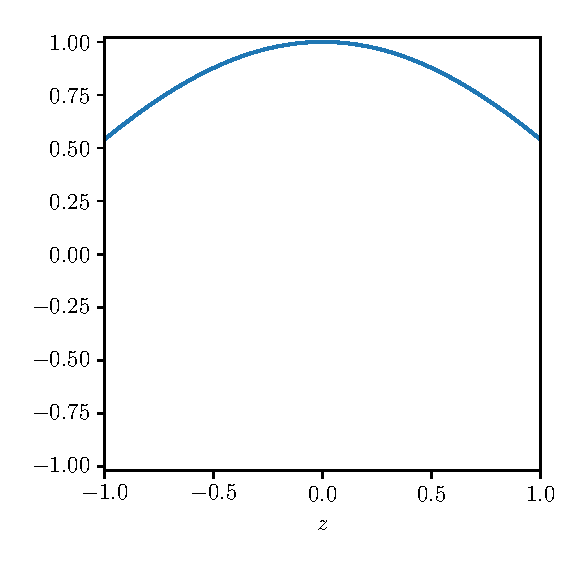
\includegraphics[width=60mm]{figures/chebyapprox_order=8.eps}
    }
    \subfloat[First derivative approximation]{
        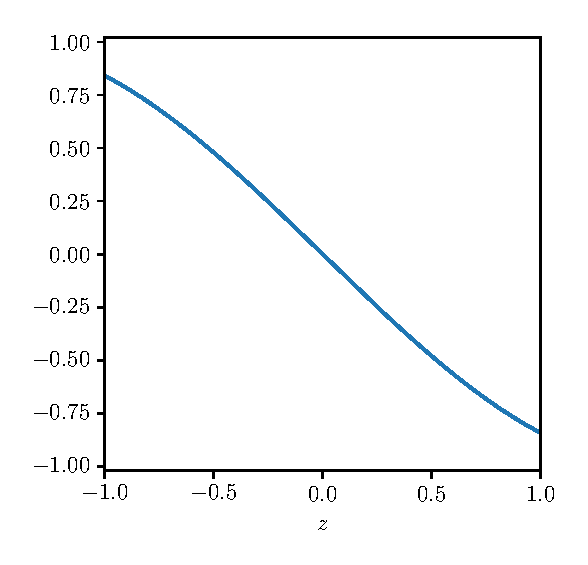
\includegraphics[width=60mm]{figures/diff1approx_order=8.eps}
    }
    \hspace{0mm}
    \subfloat[Second derivative approximation]{
        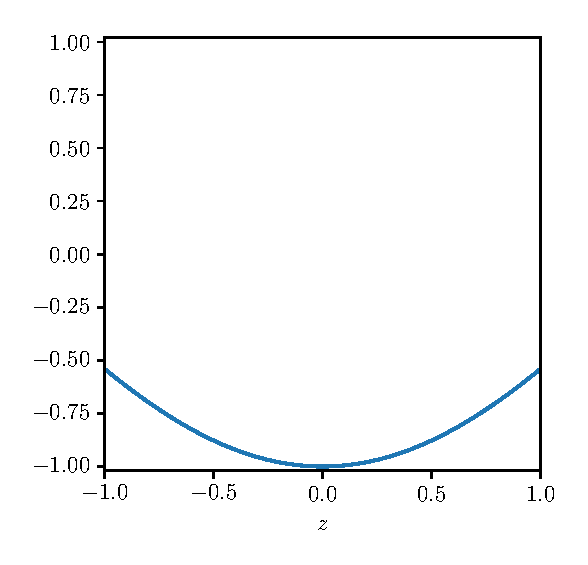
\includegraphics[width=60mm]{figures/diff2approx_order=8.eps}
    }
    \subfloat[Fourth derivative approximation]{
        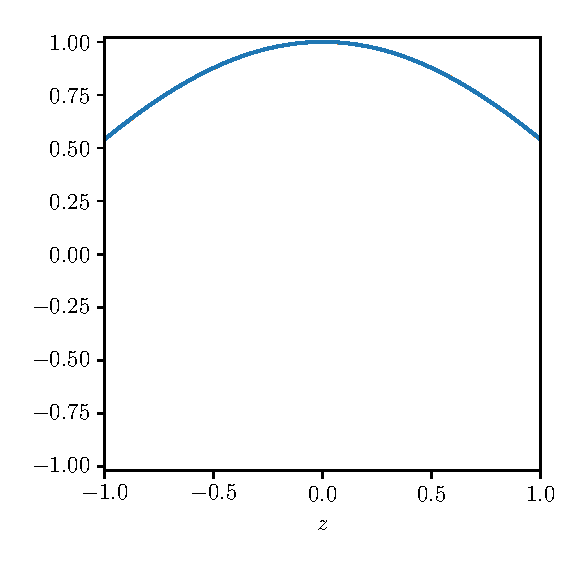
\includegraphics[width=60mm]{figures/diff4approx_order=8.eps}
    }
    \caption{The Chebyshev approximation of $ \cos(z) $ for $ N = 8 $, compared with the Chebyshev approximations of its derivatives. The (obscured) orange line in each plot corresponds to an exact derivative of $ \cos(z)$, while the blue line corresponds to the Chebyshev approximation of that derivative.}
    \label{fig:cosderivapprox}
\end{figure}

From this, we can see that this method for calculating a derivative approximation is extremely accurate. This will allow us to represent differential operators as the action of a matrix on our vector $ \mathbf{a}$. For example, the matrix $ L $ representing the action of the differential operator
\begin{equation}
    \mathcal{L} = \dv[4]{z} + 4 \dv[2]{z} - \dv[1]{z},
\end{equation} 
would have the form
\begin{equation}
    L = D^4 + 4 D^2 - D.
\end{equation}

We can now move on to discussing how we can apply these to represent the Orr-Sommerfeld equation in terms of these matrices.

\section{Fourth Order System}
To get the eigenvalues of the Orr-Sommerfeld equation we would like a generalised eigenvalue problem of the form 
\begin{equation}
    A \mathbf{a} = c B \mathbf{a},
\end{equation}
where $\mathbf{a}$ is the $ M + 1$ dimensional vector representing the coefficients of the Chebyshev expansion of our eigenfunction $ \phi$, and $ A $ and $B $ are $ (M + 1) \cross (M + 1) $ matrices.

To get matrix expressions for $A $ and $B $ we rearrange the Orr-Sommerfeld equation \eqref{oseq} to be in the following form
\begin{equation}
    (i \al R)^{-1} (D^4 - 2 \al^2 D^2 + \al^4) \p - U (D^2 - \al^2) \p + U'' \p = -c (D^2 - \al^2) \p. 
    \label{osrearrange}
\end{equation}

From here we can see that $ A $ and $ B $ take the following forms
\begin{align}
    A &= (i \al R)^{-1} (D^4 - 2 \al^2 D^2 + \al^4 I) - U (D^2 - \al^2 I) + U'' I, \\
    B &= -(D^2 - \al^2 I).
\end{align}

How do we represent our $ U $ and $ U'' $? The best way to do this is to work out some matrix that we can then multiply our coefficients for the expansion of $ \p$ and $ D^2 \p$ by \citep{bukhari1997spectral}. To do this let us assume we can accurately compute a Chebyshev expansion for our $ U $ and $ U''$ of the form
\begin{equation}
    u(z) = \sum^\infty_{j=0} b_j T_j(z).
\end{equation}

We then would like to consider the product 
\begin{align}
    h(z) &= u(z) \p(z) \\
    &= \sum^\infty_{j=0} \sum^M_{k=0} a_k b_j T_j(z) T_k(z),
    \label{chebyprod}
\end{align}
of $ 2 $ Chebyshev expansions. Can we represent the product $ T_j(z) T_k(z) $ in a nicer way? If we consider the trigonometric relation
\begin{equation}
    \cos(i \theta) \cos(j \theta) = \frac{\cos((i + j)\theta) + \cos((i - j) \theta) }{2},
\end{equation}
with $ \theta = \arccos(z)$ then we end up with the following
\begin{align}
    T_i(z) T_j(z) &= \frac{T_{i+j}(z) + T_{i-j}(z) }{2} \\
    &= \frac{T_{i+j}(z) + T_{\abs{i-j}}(z)}{2},
\end{align}
where the $ \abs{i-j}$ just comes from the fact that $ T_k(z) = T_{-k}(z) $. If we substitute this back into the product \eqref{chebyprod} we get the following
\begin{align}
    h(z) &=  \tfrac{1}{2} \sum^\infty_{j=0} \sum^M_{k = 0} a_k b_j \qb{T_{j + k}(z) + T_{\abs{j - k}}(z)} \\
    &= \tfrac{1}{2} \sum^\infty_{j=0} \sum^M_{k = 0} a_k b_j T_{j + k}(z) + \tfrac{1}{2} \sum^\infty_{j=0} \sum^M_{k = 0} a_k b_j T_{\abs{j - k}}(z).
    \label{hz}
\end{align}

If we change indices to $ n = j + k$ in the first sum, we can split the first sum into two separate sums. We have that $ b_{n - k} = 0 $ if $ n - k < 0$. This implies that if $ n < M$, we only have non-zero $ b_{n - k}$ if $ k \leq n $. If $ n > M$ we have that $ k \leq M $. This means that the following holds
\begin{equation}
    \tfrac{1}{2} \sum^\infty_{j=0} \sum^M_{k = 0} a_k b_j T_{j + k}(z) = \tfrac{1}{2} \sum^{M}_{n=0} \sum^n_{k=0} a_k b_{n - k} \T{n} + \tfrac{1}{2} \sum^\infty_{n=M} \sum^M_{k=0} a_k b_{n -k} \T{n}.
\end{equation}

For the second sum, there are two cases to consider. If $ j \leq k$ , $ \T{\abs{j - k }} = \T{k - j}$. If we substitute $ m = k - j $ then we end up with that $ m $ must take a range of between $ 0 $ and $ M$ and that $ k $ must be larger than $ m$, meaning we have the sum 
\begin{equation}
    \sum^M_{m=0} \sum^M_{k=m} a_k b_{k - m} \T{m}.
\end{equation}
If $ j > k $, if we let $ p = j - k$ we end up with the final sum 
\begin{equation}
    \sum^\infty_{p=1} \sum^M_{k=0} a_k b_{p+k} \T{p}.
\end{equation}
Notice that $ p $ starts at $ 1 $ rather than $ 0$. This is because we already have the product $ a_0 b_0 $ in the first of these two sums.

Substituting these results back into \eqref{hz} gives us our product split into $ 4 $ sums (as seen in \citet{bukhari1997spectral})
\begin{align}
    h(z) &= \tfrac{1}{2} \sum^{M}_{n=0} \sum^n_{k=0} a_k b_{n - k} \T{n} + \tfrac{1}{2} \sum^\infty_{n=M} \sum^M_{k=0} a_k b_{n -k} \T{n} \\ &+ \tfrac{1}{2} \sum^M_{n=0} \sum^M_{k=n} a_k b_{k - n} \T{n} + \tfrac{1}{2} \sum^\infty_{n=1} \sum^M_{k=0} a_k b_{n+k} \T{p},
\end{align}
where we have made the indices the same for clarity.

We can represent this product as an $ (M+1) \cross (M+1) $ matrix multiplied by a vector of the $ M + 1 $ coefficients of our function $ \p(z)$. This means each element of the matrix $ A_{nk} $ will correspond to the sum of the $ b_n $ that are multiplied by $ a_k$. For example, for $ n = 0$, we have that the first row would represent the sum
\begin{equation}
    a_0 b_0 + \tfrac{1}{2} \sum^M_{n = 1} a_n b_n,
\end{equation}
and would therefore have the row vector form
\begin{equation}
    \tfrac{1}{2} \begin{pmatrix}
        2b_0 & b_1 & b_2 & \dots & b_{M}
    \end{pmatrix}.
\end{equation}

From here on, we will represent the matrices for $ U'' $ and $ U$ by $ P $ and $ Q $ respectively as in \citet{bukhari1997spectral}.

%There are a number of methods for this. 
%In \cite{orszag1971accurate} he explicitly calculates the case for plane Poiseuille flow and therefore only has to deal with the $ z^2 $ term. Orszag computes a sum for the $k$th coefficient of $ z^2 \phi^{(n)}$ which has the following form 
% \begin{equation}
%     \tfrac{1}{4} (c_{k-2} a_{k -2}^{(n)} + (c_k + c_{k-1}) a_k^{(n)} + a_{k+2}^{(n)}).
% \end{equation}

% We can translate this into a matrix 
% \begin{equation}
%     C = \begin{pmatrix}
%         0.5 & 0 & 0.25 & 0 & 0 & 0 & 0 & \ds \\
%         0 & 0.75 & 0 & 0.25 & 0 & 0 & 0 & \ds \\
%         0.5 & 0 & 0.5 & 0 & 0.25 & 0 & 0 & \ds \\
%         0 & 0.25 & 0 & 0.5 & 0 & 0.25 & 0 & \ds \\
%         \ds & \ds & \ds & \ds & \ds & \ds & \ds & \ds
%     \end{pmatrix}.
% \end{equation}

% We can then get $ z^2 D^2 \p $ by multiplying $ D^2 \mathbf{a} $ by $ C $. Our $  U (D^2 - \al^2 I)$ then becomes $ (I - C)(D^2 - \al^2 I) $ for plane Poiseuille flow. 

% Another method is as in \cite{bukhari1997spectral} where we use matrices $ P $ and $ Q $ to represent the $ U'' $ and $ U $ terms respectively. 

For plane Poiseuille flow we have that $ U'' = -2 = -2 \T{0} $ which means that we just have that $ b_0 = -2 $ for its expansion and $ U = 1 - z^2 = \tfrac{1}{2} \T{0} - \tfrac{1}{2} \T{2} $, meaning that for the expansion of $ U $ we have that $ b_0 = \tfrac{1}{2}$ and $ b_2 = -\tfrac{1}{2} $. This means we have the following forms for $ P $ and $ Q $
\begin{equation}
    P = -2 I,\ \ Q = \begin{pmatrix}
        0.5 & 0 & -0.25 & 0 & \dots \\
        0 & 0.25 & 0 & -0.25 & \dots \\
        -0.5 & 0 & 0.5 & 0 & \dots \\
        0 & -0.25 & 0 & 0.5 & \dots \\
        \dots & \dots & \dots & \dots & \dots
    \end{pmatrix}.
\end{equation}

For Couette flow $ U'' = 0 $ and $U = z = \T{1} $, implying that $P $ and $ Q $ have the following forms
\begin{equation}
    P = 0,\ Q = \begin{pmatrix}
        0 & 0.5 & 0 & 0 & \ds \\
        1 & 0 & 0.5 & 0 & \ds \\
        0 & 0.5 & 0 & 0.5 & \ds \\
        0 & 0 & 0.5 & 0 & \ds \\
        \ds & \ds & \ds & \ds & \ds
    \end{pmatrix}.
\end{equation}

Note: When $ P $ and $ Q $ are given in \cite{bukhari1997spectral} for the case of Poiseuille flow, $ P $ is mistakenly stated to be $ 2 I $ instead of $ -2 I$ as here. 

If we use the $ P $ and $ Q $ matrices, we end up with these final forms for matrices $ A $ and $B$
\begin{align}
    A &= (i \al R)^{-1} (D^4 - 2 \al^2 D^2 + \al^4 I) - Q (D^2 - \al^2 I) + P, \\
    B &= -(D^2 - \al^2 I).
    \label{4thblockform}
\end{align}

We now have a generalised eigenvalue problem of the form $ A \mathbf{a} = c B \mathbf{a} $ which can be solved in Python. Details of exactly how this will be done are given in \ref{section:solving}.

Notice that the terms of our $ D^4 $ matrix \eqref{D4} scale with $ O(M^7) $ and the terms of our $ D^2 $ matrix \eqref{D2} scale with $ O(M^3) $. This means it is better to only use the lower-order differentiation matrices if possible. The next section will explore how to do this in the $2$nd order case. 

\section{Second Order System}
How do we make our system require only the use of $D^2$? The answer is to split the Orr-Sommerfeld equation into a system of $2$nd order equations. We define $ \phi_1 = \phi,\ \phi_2 = D^2 \phi $. These two functions allow us to represent the Orr-Sommerfeld equation \eqref{oseq} as the following system of $2$nd order differential equations
\begin{align}
    \phi_2 &= D^2 \phi_1, \\
    (i \alpha R)^{-1} ((D^2 - 2 \alpha^2) \phi_2 + \alpha^4 \phi_1) &= (U - c)(\phi_2 - \alpha^2 \phi_1) - U'' \phi_1.
    \label{2ndorder}
\end{align}

Rearrange these to get
\begin{subequations}
\begin{align}
    D^2 \phi_1 - \phi_2 &= 0, \label{2ndeq1} \\
    (U \al^2 + U'') \phi_1 + ((i \al R)^{-1} ((D^2 - 2 \al^2) - U) \phi_2 + \al^4 \phi_1) &= c \al^2 \phi_1- c\phi_2. \label{2ndeq2}
\end{align}
\end{subequations}

We want to put these into a generalised eigenvalue problem of the form $ E \mathbf{b} = c F \mathbf{b} $ like for the $4$th order case.

To begin let us work out what our vector $ \mathbf{b} $ is. If we denote the vector associated to our expansion of $ \phi_1 $ by $\mathbf{a}_1$ and the vector associated to our expansion of $ \phi_2 $ by $ \mathbf{a}_2 $ then we can form $ \mathbf{b} = (\mathbf{a}_1, \mathbf{a}_2)^\intercal $. This vector is $ 2(M+1) $ dimensional so therefore our matrices are $ 2(M+1) \cross 2(M+1) $ matrices. 

We set $E$ and $F$ out as in \cite{bukhari1997spectral}, with the first $ M + 1 $ rows corresponding to equation \eqref{2ndeq1} and the last $ M + 1 $ rows corresponding to equation \eqref{2ndeq2}. The first $ M + 1$ columns will correspond to operations done to $ \phi_1$ and the last $ M + 1 $ columns will correspond to operations done to $\phi_2$. This leaves us with the following forms for $E$ and $F$,
\begin{equation}
    E = \begin{pmatrix}
        D^2 & -I \\
        (P - \alpha^2 Q) + (i R)^{-1} \alpha^3 I & (i \alpha R)^{-1} (D^2 - 2 \alpha^2 I) - Q
    \end{pmatrix},\ \
    F = \begin{pmatrix}
        0 & 0 \\
        \alpha^2 I & -I
    \end{pmatrix}.
\label{2ndblockform}
\end{equation}

This leaves us with a generalised eigenvalue problem of the form $ E \mathbf{b} = c B \mathbf{b} $, which we can solve in the same way as our $4$th order system. Solving this should yield significantly lower numerical error than our $4$th order system. However, we can reduce the numerical error further by splitting \eqref{2ndorder} further into a system of $1$st order differential equations.

\section{First Order System}

To create a system where we only use $ D$ we need to split the Orr-Sommerfeld equation \eqref{oseq} into a system of $1$st order differential equations. To do this we define
\begin{equation} \phi_1 = \phi,\ \phi_2 = D \phi,\ \phi_3 = D^2 \phi, \phi_4 = D^3 \phi.
\label{p4}
\end{equation}

From here we have the following system of $1$st order equations
\begin{subequations}
    \begin{align}
        D \phi_1 &= \phi_2, \\
        D \phi_2 &= \phi_3, \\
        D \phi_3 &= \phi_4, \\
        (i \al R)^{-1} \phi_4 &= (i \al R)^{-1} (2 \al^2 \phi_3 - \al^4 \p_1) + (U - c)(\phi_3 - \al^2 \phi_1) - U'' \p_1.
    \end{align}
    \label{1storder}
\end{subequations}

Again we want these in the form $ G \mathbf{c} = c H \mathbf{c} $, so we rearrange the equations of \eqref{1storder} to get 
\begin{subequations}
\begin{align}
    D \p_1 - \p_2 &= 0, \\
    D \p_2 - \p_3 &= 0, \\
    D \p_3 - \p_4 &= 0, \\
    (i \al R)^{-1} D \phi_4 - (i \al R)^{-1} (2 \al^2 - U) \phi_3 + ((i \al R)^{-1} \al^4 + U \al^2  + U'') \phi_1 &= - c \phi_3 + c \al^2 \phi_1.
\end{align}
\label{1stordereq}
\end{subequations}

In the same way as the second order case, we represent the vectors corresponding to the expansions of our $4$ functions $ \p_i$ by $\mathbf{a_i} $ with $ i = 1, \dots, 4 $. We set $ \mathbf{c} = (\mathbf{a}_1, \mathbf{a}_2, \mathbf{a}_3, \mathbf{a}_4)^\intercal $. We now have a $ 4(M+1)$ dimensional vector $ \mathbf{c}$ which means that $G$ and $H$ will be $ 4(M+1) \cross 4(M+1) $ matrices.

We again follow the layout of $ G $ and $H$ as in \cite{bukhari1997spectral}. Column $ (i-1)(M+1) $ to column $ i (M+1) $ correspond to the expansion coefficients of $ \p_i $ for $ i = 1, \dots, 4$. Likewise, the rows of $G$ and $H$ are filled by the matrices corresponding to equations \eqref{1stordereq} in groups of $ M+ 1$ rows.

This leaves us with the following forms for $G$ and $H$,
\begin{equation}
    G = \begin{pmatrix}
        D & -I & 0 & 0 \\
        0 & D & -I & 0 \\
        0 & 0 & D & -I \\
        (P + \al^2 Q) + (i R)^{-1} \al^3 & 0 & -Q - (i R)^{-1} (2 \al^2) I &   (i \al R)^{-1} D
    \end{pmatrix},\ \ 
    H = \begin{pmatrix}
        0 & 0 & 0 & 0 \\
        0 & 0 & 0 & 0 \\
        0 & 0 & 0 & 0 \\
        \al^2 I & 0 & -I & 0
    \end{pmatrix}.
\label{1stblockorder}
\end{equation}

We now have a generalised eigenvalue problem $ G \mathbf{c} = c H \mathbf{c} $ that we can again solve. This system has lower numerical error than both of the other methods we have discussed but takes much longer due to the massively increased size of the matrices involved even compared to the second-order method.

\section{Boundary Conditions} \label{section:bc}
Before we can solve the resulting systems from any of our methods, we need a way to represent our boundary conditions. The Orr-Sommerfeld equation has the following boundary conditions, 
\begin{equation}
    \p(\pm 1) = \p'(\pm 1) = 0.
\end{equation}

By using the two properties \eqref{chebyprop} we get the following equations for these boundary conditions
\begin{align}
    \p(1) &=\sum^M_{k=0} a_k, \\
    \p(-1) &= \sum^M_{k=0} (-1)^k a_k, \\
    \p'(1) &= \sum^M_{k=0} k^2 a_k, \\
    \p'(-1) &= \sum^M_{k=0} (-1)^k k^2 a_k = 0.
    \label{bcsums}
\end{align}

If we combine our matrices for any of our methods with these equations we have $ M + 5 $ equations for $ M + 1 $ unknowns, meaning that our system is over-determined and only has the trivial solution $ a_k = 0 $. To solve this we follow the method that \cite{orszag1971accurate} used, to do this we $ 4 $ of the rows of our matrices with boundary equations so that we have $ M + 1 $ equations in $ M + 1 $ unknowns.

For the $4$th order system, we simply replace the last $4$ rows of $ A $ and $B$ in \eqref{4thblockform} with row vectors representing our boundary conditions in $A$ and a row of zeroes in $B$.

We follow a similar procedure for the $2$nd order case. In this case, all $4$ boundary conditions are applied to $\phi_1$ and none to $ \phi_2 $. This is because $\phi_2 = D^2 \phi $. This means the rows inserted into matrix $E$ of \eqref{2ndblockform} will be of the form $ (\mathbf{v}, \mathbf{0})$ where $ \mathbf{v}$ is the $ M+1 $ dimensional vector representing one of the $4$ sums given in \eqref{bcsums} and $\mathbf{0} $ is the $ M +1 $ dimensional zero vector. 

We replace the $ (M - 1)th,\ Mth,\ 2(M-1)th \text{ and } 2Mth$ rows of $E$ and $F$. As with the $4$th order case, the rows replaced in $F$ are just replaced with rows of zeroes. The specific order of how the rows are inserted does not matter \citep{bukhari1997spectral}.

Finally, we deal with the $1$st order system. In this case, we apply the first two boundary conditions to $ \phi_1 $ and the first two boundary conditions again to $ \phi_2$. This is because $ \phi_2 $ represents the first derivative of $ \phi $ and therefore we don't need to apply the boundary conditions that fix the derivative of a function. 

The rows representing the boundary conditions applied to $\phi_1$ have the form $ (\mathbf{v}, \mathbf{0}, \mathbf{0}, \mathbf{0}) $ and the rows representing the boundary conditions applied to $ \phi_2 $ have the form $ (\mathbf{0}, \mathbf{v}, \mathbf{0}, \mathbf{0}) $. They are inserted into the $Mth,\ 2Mth,\ 3Mth\ \text{and}\ 4Mth$ rows of $ G $ and $H$. Again we insert just rows of zeroes into $H$.

We now can move on to solving our systems.

\section{Solving our system} \label{section:solving}
For each of the above methods we now have a generalised eigenvalue problem of the form
\begin{equation}
    A \mathbf{b} = c B \mathbf{b}.
    \label{geneigproblem}
\end{equation}
We implement this system in Python (the code for this is found in the appendix), but we have a problem! The matrix $ B $ is singular due to the rows of zeros added by the boundary conditions, which means we cannot rearrange \eqref{geneigproblem} to be in the form $ A B^{-1} \mathbf{b} = c \mathbf{b} $ and therefore cannot be solved using just any eigenvalue method. 

To solve them we use the QZ algorithm of \cite{moler1973algorithm}, as suggested by \cite{dongarra1996chebyshev} which allows us to get the eigenvalues of this problem even though the matrix $ B $ is singular. In Python, this is implemented in the \codeword{scipy.linalg.eig} function in the \codeword{scipy} package, a link to which is found \href{https://docs.scipy.org/doc/scipy/reference/generated/scipy.linalg.eig.html}{\textcolor{blue}{here}}. 

The reason that the QZ algorithm is preferred is two-fold. Firstly, the QZ algorithm can find all of the eigenvalues of the system \eqref{geneigproblem} and does not require knowledge of the position of the eigenvalues as with shooting or search methods. This is useful for this case as we are searching for any eigenvalue with an imaginary part above $0$ and therefore want all possible eigenvalues of our system. Secondly, as shown in \cite{dongarra1996chebyshev}, using a search technique such as \cite{orszag1971accurate} can 'miss out' eigenvalues. 

The QZ algorithm transforms $A $ and $B$ using Householder transformations and then calculates their eigenvalues as $ \al_i$ and $ \beta_i$, where the $ \al_i$ are the eigenvalues of $A $ and the $ \beta_i$ are the eigenvalues of $ B$. The eigenvalues of our system are then obtained by dividing each $ \al_i$ by its respective $ \beta_i$. As our system is singular, we would expect some of our eigenvalues to be 'infinite' or 'spurious' eigenvalues caused by this singularity. An additional advantage of the QZ algorithm is that we can filter out these 'spurious' eigenvalues by checking the $ \beta_i$. Specifically, we remove any that are zero.

We now have several numerical methods implemented that can be used to assess the stability of flows for various values of $ R $. The focus of the next chapter will be on the results that we obtain along with a comparison of the numerical accuracy of these methods.

\section{Chebyshev Tau method}

It's also worth mentioning why this is referred to as the Chebyshev Tau method. This is because this method doesn't exactly solve the Orr-Sommerfeld equation, but exactly solves the Orr-Sommerfeld equation with the following additional terms on the right-hand side (in the fourth order case)
\begin{equation}
    \tau_1 \T{M-3} + \tau_2 \T{M-2} + \tau_3 \T{M-1} + \tau_4 \T{M}.
\end{equation}

These $ \tau_i$ can be used to get error bounds if this method is used to get a solution to a differential equation \citep{fox1968chebyshev}, but cannot be used in this way if used to solve for eigenvalues as we are doing here. 

In the case of the second-order and first-order methods, they are actually solving their systems of equations with two tau coefficients on the right-hand side in the second-order case and one tau coefficient on the left-hand side in the first-order case. Since the approximation converges \citet{orszag1971accurate}, we have a strong implication that the higher-order methods are more accurate. Part of the next chapter will be verifying that this is the case.

The tau method was first derived by \citet{lanczos1988applied}.